\documentclass{article}
\usepackage[a4paper,margin=2cm]{geometry}
\title{Analysis Summary}
\author{generated with CAFCore/CommonAnalysisHelpers by user bjager}
\date{09-06-2022}
\usepackage{adjustbox}
\usepackage{graphicx}
\usepackage[subpreambles]{standalone}
\usepackage{fancyhdr}
\pagestyle{fancy}
\setcounter{secnumdepth}{0}
\usepackage{tikz}
\usetikzlibrary{positioning,arrows}
\usepackage{hyperref}
\usepackage[open]{bookmark}
\begin{document}
\maketitle
\tableofcontents

\begin{itemize}
\item \textbf{prepare} was run on \textbf{Tue Sep 28 09:53:31 2021} compiled with gcc 8.3.0 under ROOT 6.18/04 using the configuration \textbf{'config/master/VBF/prepare-VBF-default.cfg'} with options \textbf{'outputFile=sampleFolders/prepared/210924-samples-prepared.root'} \item \textbf{initialize} was run on \textbf{Tue Sep 28 11:15:28 2021} compiled with gcc 8.3.0 under ROOT 6.18/04 using the configuration \textbf{'config/master/VBF/initialize-VBF-default.cfg'} with options \textbf{'outputFile=/project/ctb-stelzer/bjager/CAFoutput/batchOutput/unmerged\_210928-initialized-nom/unmerged\_210928-initialized-nom\_sig\_X\_c16e\_vh.root', 'inputFile=sampleFolders/prepared/210924-samples-prepared.root', 'campaignsConfig=config/master/common/campaigns-cedar-V21-PFlowJets-skimmed.cfg', 'prettyPrint=false', 'lineUpdates=false', 'prettyPrint=false', 'lineUpdates=false', 'prettyPrint=false', 'lineUpdates=false', 'prettyPrint=false', 'lineUpdates=false', 'prettyPrint=false', 'lineUpdates=false', 'prettyPrint=false', 'lineUpdates=false', 'prettyPrint=false', 'lineUpdates=false', 'prettyPrint=false', 'lineUpdates=false', 'prettyPrint=false', 'lineUpdates=false', 'prettyPrint=false', 'lineUpdates=false', 'prettyPrint=false', 'lineUpdates=false', 'prettyPrint=false', 'lineUpdates=false', 'prettyPrint=false', 'lineUpdates=false', 'prettyPrint=false', 'lineUpdates=false', 'prettyPrint=false', 'lineUpdates=false', 'prettyPrint=false', 'lineUpdates=false', 'prettyPrint=false', 'lineUpdates=false', 'prettyPrint=false', 'lineUpdates=false', 'prettyPrint=false', 'lineUpdates=false', 'prettyPrint=false', 'lineUpdates=false', 'prettyPrint=false', 'lineUpdates=false', 'prettyPrint=false', 'lineUpdates=false', 'prettyPrint=false', 'lineUpdates=false', 'prettyPrint=false', 'lineUpdates=false', 'prettyPrint=false', 'lineUpdates=false', 'prettyPrint=false', 'lineUpdates=false', 'prettyPrint=false', 'lineUpdates=false', 'prettyPrint=false', 'lineUpdates=false', 'prettyPrint=false', 'lineUpdates=false', 'prettyPrint=false', 'lineUpdates=false', 'prettyPrint=false', 'lineUpdates=false', 'prettyPrint=false', 'lineUpdates=false', 'prettyPrint=false', 'lineUpdates=false', 'prettyPrint=false', 'lineUpdates=false', 'prettyPrint=false', 'lineUpdates=false', 'prettyPrint=false', 'lineUpdates=false', 'prettyPrint=false', 'lineUpdates=false', 'prettyPrint=false', 'lineUpdates=false', 'prettyPrint=false', 'lineUpdates=false', 'prettyPrint=false', 'lineUpdates=false', 'prettyPrint=false', 'lineUpdates=false', 'prettyPrint=false', 'lineUpdates=false', 'prettyPrint=false', 'lineUpdates=false', 'prettyPrint=false', 'lineUpdates=false', 'prettyPrint=false', 'lineUpdates=false', 'prettyPrint=false', 'lineUpdates=false', 'inputFile=sampleFolders/prepared/210924-samples-prepared.root', 'campaignsConfig=config/master/common/campaigns-cedar-V21-PFlowJets-skimmed.cfg'} \item \textbf{analyze} was run on \textbf{Wed Sep 29 17:55:57 2021} compiled with gcc 8.3.0 under ROOT 6.18/04 using the configuration \textbf{'config/master/STXS/analyze-VBF-STXS-nominal.cfg'} with options \textbf{'outputFile=/project/ctb-stelzer/bjager/CAFoutput/batchOutput/unmerged\_210924-VBF-nom-4/unmerged\_210924-VBF-nom-4\_sig\_X\_X\_vh.part6.root', 'inputFile=sampleFolders/initialized/210928-samples-initialized-nom.root', 'prettyPrint=false', 'lineUpdates=false', 'prettyPrint=false', 'lineUpdates=false', 'prettyPrint=false', 'lineUpdates=false', 'prettyPrint=false', 'lineUpdates=false', 'prettyPrint=false', 'lineUpdates=false', 'inputFile=sampleFolders/initialized/210928-samples-initialized-nom.root'} \item \textbf{visualize} was run on \textbf{Thu Jun  9 14:08:52 2022} compiled with gcc 8.3.0 under ROOT 6.18/04 using the configuration \textbf{'config/master/VBF/visualize-VBF-default.cfg'} with options \textbf{'inputFile=/project/ctb-stelzer/bjager/CAFoutput/FullRun2PaperWorkspaces/210924-4-samples-analyzed-VBF-nom.root', 'outputDir=results/220605-Thesis/topcr/lepcent', 'doNFs=false', 'makePlots=CutVBF\_TopControl\_2jet/contOLV', 'makeLogPlots=true', 'histogramProcesses=config/visualization/processes/VBF/prefit-nfs-TopCR.txt', 'patches=config/visualization/style/VBF/VBF-style-post-fit-noLines.txt', 'plotter.geometry.legend.xMin=0.52', 'plotter.geometry.legend.yMin=0.7', 'plotter.geometry.legend.xMax=0.91', 'plotter.geometry.legend.yMax=0.92', 'plotter.legend.showTotalBkgErrorType=false', 'plotter.legend.showTotalBkgErrorType=false', 'plotter.style.legend.showTotalBkgErrorType=false', 'geometry.main.yAxis.titleOffset=1.2', 'plotter.style.legend.errorDisplayType=f', 'plotter.style.listSignalFirst=true', 'plotter.style.stackSignal=true', 'plotter.style.manualStacking=true', 'plotter.style.reverseStacking=true', 'plotter.style.unsorted=true', 'plotter.style.listDataFirst=true', 'plotter.style.nLegendCols=2', 'plotter.style.sub.yAxis.nDiv=505', 'plotter.style.main.totalStackError.fillStyle=3245', 'plotter.style.ratioMax=1.45', 'plotter.style.ratioMin=0.55', 'plotter.style.legend.textSize=0.03', 'plotter.style.min=0', 'plotter.style.autoStackLegend=true', 'plotter.style.autoStackSignal=true', 'plotter.labels.legendTotalBkg=Uncertainty', 'plotter.labels.drawInfo=false', 'plotter.style.main.totalStack.lineWidth=0', 'plotter.style.main.totalStack.lineColor=kWhite', 'plotter.style.sub.margin=1.2', 'plotter.style.labels.yPos=0.93', 'plotter.style.labels.xOffset=0.19', 'plotter.legend.dataDisplayType=lep', 'plotter.style.forceRatioLimits=true', 'plotter.style.showOverflow=true', 'plotter.labels.totalStack=Pred.', 'plotter.labels.drawATLAS=false', 'labels.drawATLAS=false', 'plotter.style.labels.drawATLAS=false', 'plotter.style.showRatio=true', 'plotter.style.max.scale=1', 'makeCutflows=false', 'systematicsBands=auxData/systematicsBands/VBF/210927-systematics-reduced-band-file.root:systematics>>::emme', 'plotter.errors.showSys=emme', 'plotter.errors.source=totalStack', 'plotter.errors.shiftTo=totalStack', 'plotter.errors.normSys=true', 'plotter.errors.shapeSys=false', 'plotter.verbose=false', 'plotter.labels.axes.subX=C\_{l1} + C\_{l2}'} \end{itemize}
\section[Cut Overview]{Cut Overview}

\centering

\adjustbox{width=\textwidth,height=\textheight,keepaspectratio}{\documentclass{standalone}
\usepackage{tikz}
\usepackage{underscore}
\usepackage[T1]{fontenc}
\usetikzlibrary{positioning,arrows}
\begin{document}
\begingroup
\tikzstyle{block} = [rectangle, draw, fill=blue!20, text width=10em, inner sep=2.5pt, text centered, rounded corners, minimum height=2em]
\tikzstyle{job} = [rectangle, draw, fill=red!20, inner sep=2.5pt, rounded corners, font={\tiny}]
\tikzstyle{line} = [draw, -latex']

\begin{tikzpicture}[]
\node [block] (basecut) {__baseCut__};
\node [block, below=of basecut] (cutstxs) {Signal split into STXS bins};
\node [block, below=of cutstxs] (cutchannels) {Channel Selection};
\node [block, below=of cutchannels] (cuttrigger) {Trigger Selection};
\node [block, below=of cuttrigger] (cuttriggermatch) {Trigger Matching};
\node [block, below=of cuttriggermatch] (cutdatadrivenmufake) {W+jets flavour split muon};
\node [block, below=of cutdatadrivenmufake] (cutdatadrivenelfake) {W+jets flavour split electron};
\node [block, below=of cutdatadrivenelfake] (cutjetcleaning) {Jet Cleaning};
\node [block, below=of cutjetcleaning] (cutvgammavjetoverlap) {Overlap: Vgamma/Vjets};
\node [block, below=of cutvgammavjetoverlap] (cut2leptons) {Only two Leptons};
\node [block, below=of cut2leptons] (cutleadleptonpt) {$p_{t}^{lead} > 22$ GeV};
\node [block, below=of cutleadleptonpt] (cutsubleadleptonpt) {$p_{t}^{\rm sublead} > 15$};
\node [block, below=of cutsubleadleptonpt] (cutremovehigheventweights) {Remove High Eventweight Events};
\node [block, below=of cutremovehigheventweights] (cutosleptons) {OS Leptons};
\node [block, below=of cutosleptons] (cutmll) {$M_{\ell\ell} > 12/10$ GeV};
\node [block, below=of cutmll] (cutzveto) {SF: Z Veto};
\node [block, below=of cutzveto] (cutlepselection) {Leptons ID, singleFakes 1 anti-ID,1 ID, doubleFakes 2*anti-ID};
\node [block, below=of cutlepselection] (cutqcdff) {Apply QCD FF weight};
\node [block, below=of cutqcdff] (cutff) {Apply fake factor};
\node [block, below=of cutff] (cutvbf2jet) {2-jet (30,30) fJVT};
\node [block, below=of cutvbf2jet] (cutvbfbveto2jet) {b-veto};
\node [block, below=of cutvbfbveto2jet] (cutvbfztautaucontrolbveto2jet) {$Z\to\tau\tau$ CR: $\vert m_{\tau\tau}-m_Z\vert<$ 25, bVeto};
\node [block, below=of cutvbfztautaucontrolbveto2jet] (cutvbfztautaucontrolbveto2jetmllmet) {$Z\to\tau\tau$ CR: $M_{ll}<70$ GeV};
\node [block, below=of cutvbfztautaucontrolbveto2jetmllmet] (cutvbfztautaucontrol2jetinclcjv) {$Z\to\tau\tau$ CR: CJV$<30$ GeV};
\node [block, below=of cutvbfztautaucontrol2jetinclcjv] (cutvbfztautaucontrol2jetinclolv) {$Z\to\tau\tau$ CR: OLV};
\node [block, below=of cutvbfztautaucontrol2jetinclolv] (cutvbfztautaucontrol2jet) {Ztautau CR};
\node [block, below=of cutvbfztautaucontrol2jet] (cutvbfztautaucontrol2jetmjjgt350) {qq2Hqq_MJJ_GT350};
\node [block, below=of cutvbfztautaucontrol2jetmjjgt350] (cutvbfztautaucontrol2jetmjjgt350pth0200) {ZttCR_qq2Hqq_2J_PTH_0_200};
\node [block, below=of cutvbfztautaucontrol2jetmjjgt350pth0200] (cutvbfztautaucontrol2jetmjjgt700pth0200) {ZttCR_qq2Hqq_2J_MJJ_GT700_PTH_0_200};
\node [block, below=of cutvbfztautaucontrol2jetmjjgt700pth0200] (cutvbfztautaucontrol2jetmjj10001500pth0200) {ZttCR_qq2Hqq_2J_MJJ_1000_1500_PTH_0_200};
\node [block, below=of cutvbfztautaucontrol2jetmjj10001500pth0200] (cutvbfztautaucontrol2jetmjj10001500pth0200pthjj025) {ZttCR_qq2Hqq_2J_MJJ_1000_1500_PTH_0_200_PTHJJ_0_25};
\path [line] (node cs:name=cutvbfztautaucontrol2jetmjj10001500pth0200, anchor=south) -| (node cs:name=cutvbfztautaucontrol2jetmjj10001500pth0200pthjj025, anchor=north);
\node [block, right=1*0.1cm+0*(10em+2*2.5pt) of cutvbfztautaucontrol2jetmjj10001500pth0200pthjj025] (cutvbfztautaucontrol2jetmjj10001500pth0200pthjjgt25) {ZttCR_qq2Hqq_2J_MJJ_1000_1500_PTH_0_200_PTHJJ_GT25};
\path [line] (node cs:name=cutvbfztautaucontrol2jetmjj10001500pth0200, anchor=east) -| (node cs:name=cutvbfztautaucontrol2jetmjj10001500pth0200pthjjgt25, anchor=north);
\path [line] (node cs:name=cutvbfztautaucontrol2jetmjjgt700pth0200, anchor=south) -| (node cs:name=cutvbfztautaucontrol2jetmjj10001500pth0200, anchor=north);
\node [block, right=2*0.1cm+1*(10em+2*2.5pt) of cutvbfztautaucontrol2jetmjj10001500pth0200] (cutvbfztautaucontrol2jetmjjgt1500pth0200) {ZttCR_qq2Hqq_2J_MJJ_GT1500_PTH_0_200};
\node [block, below=of cutvbfztautaucontrol2jetmjjgt1500pth0200] (cutvbfztautaucontrol2jetmjjgt1500pth0200pthjj025) {ZttCR_qq2Hqq_2J_MJJ_GT1500_PTH_0_200_PTHJJ_0_25};
\path [line] (node cs:name=cutvbfztautaucontrol2jetmjjgt1500pth0200, anchor=south) -| (node cs:name=cutvbfztautaucontrol2jetmjjgt1500pth0200pthjj025, anchor=north);
\node [block, right=1*0.1cm+0*(10em+2*2.5pt) of cutvbfztautaucontrol2jetmjjgt1500pth0200pthjj025] (cutvbfztautaucontrol2jetmjjgt1500pth0200pthjjgt25) {ZttCR_qq2Hqq_2J_MJJ_GT1500_PTH_0_200_PTHJJ_GT25};
\path [line] (node cs:name=cutvbfztautaucontrol2jetmjjgt1500pth0200, anchor=east) -| (node cs:name=cutvbfztautaucontrol2jetmjjgt1500pth0200pthjjgt25, anchor=north);
\path [line] (node cs:name=cutvbfztautaucontrol2jetmjjgt700pth0200, anchor=east) -| (node cs:name=cutvbfztautaucontrol2jetmjjgt1500pth0200, anchor=north);
\node [block, right=2*0.1cm+1*(10em+2*2.5pt) of cutvbfztautaucontrol2jetmjjgt1500pth0200] (cutvbfztautaucontrol2jetmjj7001000pth0200) {ZttCR_qq2Hqq_2J_MJJ_700_1000_PTH_0_200};
\node [block, below=of cutvbfztautaucontrol2jetmjj7001000pth0200] (cutvbfztautaucontrol2jetmjj7001000pth0200pthjj025) {ZttCR_qq2Hqq_2J_MJJ_700_1000_PTH_0_200_PTHJJ_0_25};
\path [line] (node cs:name=cutvbfztautaucontrol2jetmjj7001000pth0200, anchor=south) -| (node cs:name=cutvbfztautaucontrol2jetmjj7001000pth0200pthjj025, anchor=north);
\node [block, right=1*0.1cm+0*(10em+2*2.5pt) of cutvbfztautaucontrol2jetmjj7001000pth0200pthjj025] (cutvbfztautaucontrol2jetmjj7001000pth0200pthjjgt25) {ZttCR_qq2Hqq_2J_MJJ_700_1000_PTH_0_200_PTHJJ_GT25};
\path [line] (node cs:name=cutvbfztautaucontrol2jetmjj7001000pth0200, anchor=east) -| (node cs:name=cutvbfztautaucontrol2jetmjj7001000pth0200pthjjgt25, anchor=north);
\path [line] (node cs:name=cutvbfztautaucontrol2jetmjjgt700pth0200, anchor=east) -| (node cs:name=cutvbfztautaucontrol2jetmjj7001000pth0200, anchor=north);
\path [line] (node cs:name=cutvbfztautaucontrol2jetmjjgt350pth0200, anchor=south) -| (node cs:name=cutvbfztautaucontrol2jetmjjgt700pth0200, anchor=north);
\node [block, right=6*0.1cm+5*(10em+2*2.5pt) of cutvbfztautaucontrol2jetmjjgt700pth0200] (cutvbfztautaucontrol2jetmjj350700pth0200) {ZttCR_qq2Hqq_2J_MJJ_350_700_PTH_0_200};
\node [block, below=of cutvbfztautaucontrol2jetmjj350700pth0200] (cutvbfztautaucontrol2jetmjj350700pth0200pthjj025) {ZttCR_qq2Hqq_2J_MJJ_350_700_PTH_0_200_PTHJJ_0_25};
\path [line] (node cs:name=cutvbfztautaucontrol2jetmjj350700pth0200, anchor=south) -| (node cs:name=cutvbfztautaucontrol2jetmjj350700pth0200pthjj025, anchor=north);
\node [block, right=1*0.1cm+0*(10em+2*2.5pt) of cutvbfztautaucontrol2jetmjj350700pth0200pthjj025] (cutvbfztautaucontrol2jetmjj350700pth0200pthjjgt25) {ZttCR_qq2Hqq_2J_MJJ_350_700_PTH_0_200_PTHJJ_GT25};
\path [line] (node cs:name=cutvbfztautaucontrol2jetmjj350700pth0200, anchor=east) -| (node cs:name=cutvbfztautaucontrol2jetmjj350700pth0200pthjjgt25, anchor=north);
\path [line] (node cs:name=cutvbfztautaucontrol2jetmjjgt350pth0200, anchor=east) -| (node cs:name=cutvbfztautaucontrol2jetmjj350700pth0200, anchor=north);
\path [line] (node cs:name=cutvbfztautaucontrol2jetmjjgt350, anchor=south) -| (node cs:name=cutvbfztautaucontrol2jetmjjgt350pth0200, anchor=north);
\node [block, right=8*0.1cm+7*(10em+2*2.5pt) of cutvbfztautaucontrol2jetmjjgt350pth0200] (cutvbfztautaucontrol2jetmjjgt350pthgt200) {ZttCR_qq2Hqq_2J_PTH_GT200};
\node [block, below=of cutvbfztautaucontrol2jetmjjgt350pthgt200] (cutvbfztautaucontrol2jetmjj7001000pthgt200) {ZttCR_qq2Hqq_2J_MJJ_700_1000_PTH_GT200};
\node [block, below=of cutvbfztautaucontrol2jetmjj7001000pthgt200] (cutvbfztautaucontrol2jetmjj7001000pthgt200pthjj025) {ZttCR_qq2Hqq_2J_MJJ_700_1000_PTH_GT200_PTHJJ_0_25};
\path [line] (node cs:name=cutvbfztautaucontrol2jetmjj7001000pthgt200, anchor=south) -| (node cs:name=cutvbfztautaucontrol2jetmjj7001000pthgt200pthjj025, anchor=north);
\node [block, right=1*0.1cm+0*(10em+2*2.5pt) of cutvbfztautaucontrol2jetmjj7001000pthgt200pthjj025] (cutvbfztautaucontrol2jetmjj7001000pthgt200pthjjgt25) {ZttCR_qq2Hqq_2J_MJJ_700_1000_PTH_GT200_PTHJJ_GT25};
\path [line] (node cs:name=cutvbfztautaucontrol2jetmjj7001000pthgt200, anchor=east) -| (node cs:name=cutvbfztautaucontrol2jetmjj7001000pthgt200pthjjgt25, anchor=north);
\path [line] (node cs:name=cutvbfztautaucontrol2jetmjjgt350pthgt200, anchor=south) -| (node cs:name=cutvbfztautaucontrol2jetmjj7001000pthgt200, anchor=north);
\node [block, right=2*0.1cm+1*(10em+2*2.5pt) of cutvbfztautaucontrol2jetmjj7001000pthgt200] (cutvbfztautaucontrol2jetmjj350700pthgt200) {ZttCR_qq2Hqq_2J_MJJ_350_700_PTH_GT200};
\node [block, below=of cutvbfztautaucontrol2jetmjj350700pthgt200] (cutvbfztautaucontrol2jetmjj350700pthgt200pthjj025) {ZttCR_qq2Hqq_2J_MJJ_350_700_PTH_GT200_PTHJJ_0_25};
\path [line] (node cs:name=cutvbfztautaucontrol2jetmjj350700pthgt200, anchor=south) -| (node cs:name=cutvbfztautaucontrol2jetmjj350700pthgt200pthjj025, anchor=north);
\node [block, right=1*0.1cm+0*(10em+2*2.5pt) of cutvbfztautaucontrol2jetmjj350700pthgt200pthjj025] (cutvbfztautaucontrol2jetmjj350700pthgt200pthjjgt25) {ZttCR_qq2Hqq_2J_MJJ_350_700_PTH_GT200_PTHJJ_GT25};
\path [line] (node cs:name=cutvbfztautaucontrol2jetmjj350700pthgt200, anchor=east) -| (node cs:name=cutvbfztautaucontrol2jetmjj350700pthgt200pthjjgt25, anchor=north);
\path [line] (node cs:name=cutvbfztautaucontrol2jetmjjgt350pthgt200, anchor=east) -| (node cs:name=cutvbfztautaucontrol2jetmjj350700pthgt200, anchor=north);
\node [block, right=2*0.1cm+1*(10em+2*2.5pt) of cutvbfztautaucontrol2jetmjj350700pthgt200] (cutvbfztautaucontrol2jetmjjgt1500pthgt200) {ZttCR_qq2Hqq_2J_MJJ_GT1500_PTH_GT200};
\node [block, below=of cutvbfztautaucontrol2jetmjjgt1500pthgt200] (cutvbfztautaucontrol2jetmjjgt1500pthgt200pthjj025) {ZttCR_qq2Hqq_2J_MJJ_GT1500_PTH_GT200_PTHJJ_0_25};
\path [line] (node cs:name=cutvbfztautaucontrol2jetmjjgt1500pthgt200, anchor=south) -| (node cs:name=cutvbfztautaucontrol2jetmjjgt1500pthgt200pthjj025, anchor=north);
\node [block, right=1*0.1cm+0*(10em+2*2.5pt) of cutvbfztautaucontrol2jetmjjgt1500pthgt200pthjj025] (cutvbfztautaucontrol2jetmjjgt1500pthgt200pthjjgt25) {ZttCR_qq2Hqq_2J_MJJ_GT1500_PTH_GT200_PTHJJ_GT25};
\path [line] (node cs:name=cutvbfztautaucontrol2jetmjjgt1500pthgt200, anchor=east) -| (node cs:name=cutvbfztautaucontrol2jetmjjgt1500pthgt200pthjjgt25, anchor=north);
\path [line] (node cs:name=cutvbfztautaucontrol2jetmjjgt350pthgt200, anchor=east) -| (node cs:name=cutvbfztautaucontrol2jetmjjgt1500pthgt200, anchor=north);
\node [block, right=2*0.1cm+1*(10em+2*2.5pt) of cutvbfztautaucontrol2jetmjjgt1500pthgt200] (cutvbfztautaucontrol2jetmjj10001500pthgt200) {ZttCR_qq2Hqq_2J_MJJ_1000_1500_PTH_GT200};
\node [block, below=of cutvbfztautaucontrol2jetmjj10001500pthgt200] (cutvbfztautaucontrol2jetmjj10001500pthgt200pthjj025) {ZttCR_qq2Hqq_2J_MJJ_1000_1500_PTH_GT200_PTHJJ_0_25};
\path [line] (node cs:name=cutvbfztautaucontrol2jetmjj10001500pthgt200, anchor=south) -| (node cs:name=cutvbfztautaucontrol2jetmjj10001500pthgt200pthjj025, anchor=north);
\node [block, right=1*0.1cm+0*(10em+2*2.5pt) of cutvbfztautaucontrol2jetmjj10001500pthgt200pthjj025] (cutvbfztautaucontrol2jetmjj10001500pthgt200pthjjgt25) {ZttCR_qq2Hqq_2J_MJJ_1000_1500_PTH_GT200_PTHJJ_GT25};
\path [line] (node cs:name=cutvbfztautaucontrol2jetmjj10001500pthgt200, anchor=east) -| (node cs:name=cutvbfztautaucontrol2jetmjj10001500pthgt200pthjjgt25, anchor=north);
\path [line] (node cs:name=cutvbfztautaucontrol2jetmjjgt350pthgt200, anchor=east) -| (node cs:name=cutvbfztautaucontrol2jetmjj10001500pthgt200, anchor=north);
\path [line] (node cs:name=cutvbfztautaucontrol2jetmjjgt350, anchor=east) -| (node cs:name=cutvbfztautaucontrol2jetmjjgt350pthgt200, anchor=north);
\path [line] (node cs:name=cutvbfztautaucontrol2jet, anchor=south) -| (node cs:name=cutvbfztautaucontrol2jetmjjgt350, anchor=north);
\path [line] (node cs:name=cutvbfztautaucontrol2jetinclolv, anchor=south) -| (node cs:name=cutvbfztautaucontrol2jet, anchor=north);
\node [block, right=16*0.1cm+15*(10em+2*2.5pt) of cutvbfztautaucontrol2jet] (cutvbfztautaucontrol25dnn52) {0.25 <  DNN < 0.52};
\path [line] (node cs:name=cutvbfztautaucontrol2jetinclolv, anchor=east) -| (node cs:name=cutvbfztautaucontrol25dnn52, anchor=north);
\node [block, right=1*0.1cm+0*(10em+2*2.5pt) of cutvbfztautaucontrol25dnn52] (cutvbfztautaucontroldnn68) {DNN > 0.68};
\path [line] (node cs:name=cutvbfztautaucontrol2jetinclolv, anchor=east) -| (node cs:name=cutvbfztautaucontroldnn68, anchor=north);
\node [block, right=1*0.1cm+0*(10em+2*2.5pt) of cutvbfztautaucontroldnn68] (cutvbfztautaucontroldnn25) {DNN > 0.25};
\path [line] (node cs:name=cutvbfztautaucontrol2jetinclolv, anchor=east) -| (node cs:name=cutvbfztautaucontroldnn25, anchor=north);
\node [block, right=1*0.1cm+0*(10em+2*2.5pt) of cutvbfztautaucontroldnn25] (cutvbfztautaucontroldnn52) {DNN > 0.52};
\path [line] (node cs:name=cutvbfztautaucontrol2jetinclolv, anchor=east) -| (node cs:name=cutvbfztautaucontroldnn52, anchor=north);
\node [block, right=1*0.1cm+0*(10em+2*2.5pt) of cutvbfztautaucontroldnn52] (cutvbfztautaucontrol2jetinclolvtightermll) {$M_{ll}<60$ GeV};
\path [line] (node cs:name=cutvbfztautaucontrol2jetinclolv, anchor=east) -| (node cs:name=cutvbfztautaucontrol2jetinclolvtightermll, anchor=north);
\node [block, right=1*0.1cm+0*(10em+2*2.5pt) of cutvbfztautaucontrol2jetinclolvtightermll] (cutvbfztautaucontroldnncut41) {DNN > 0.25};
\path [line] (node cs:name=cutvbfztautaucontrol2jetinclolv, anchor=east) -| (node cs:name=cutvbfztautaucontroldnncut41, anchor=north);
\node [block, right=1*0.1cm+0*(10em+2*2.5pt) of cutvbfztautaucontroldnncut41] (cutvbfztautaucontrolmtormt2) {$M_{T}$<130 GeV || $M_{T2}$<160 GeV};
\path [line] (node cs:name=cutvbfztautaucontrol2jetinclolv, anchor=east) -| (node cs:name=cutvbfztautaucontrolmtormt2, anchor=north);
\node [block, right=1*0.1cm+0*(10em+2*2.5pt) of cutvbfztautaucontrolmtormt2] (cutvbfztautaucontrol25dnn) {DNN < 0.25};
\path [line] (node cs:name=cutvbfztautaucontrol2jetinclolv, anchor=east) -| (node cs:name=cutvbfztautaucontrol25dnn, anchor=north);
\node [block, right=1*0.1cm+0*(10em+2*2.5pt) of cutvbfztautaucontrol25dnn] (cutvbfztautaucontroldnncut42) {DNN > 0.01};
\path [line] (node cs:name=cutvbfztautaucontrol2jetinclolv, anchor=east) -| (node cs:name=cutvbfztautaucontroldnncut42, anchor=north);
\path [line] (node cs:name=cutvbfztautaucontrol2jetinclcjv, anchor=south) -| (node cs:name=cutvbfztautaucontrol2jetinclolv, anchor=north);
\node [block, right=25*0.1cm+24*(10em+2*2.5pt) of cutvbfztautaucontrol2jetinclolv] (cutvbfztautaucontrol2jetincltightermll) {$M_{ll}<60$ GeV};
\node [block, below=of cutvbfztautaucontrol2jetincltightermll] (cutvbfztautaucontroldnncut32) {DNN > 0.01};
\path [line] (node cs:name=cutvbfztautaucontrol2jetincltightermll, anchor=south) -| (node cs:name=cutvbfztautaucontroldnncut32, anchor=north);
\path [line] (node cs:name=cutvbfztautaucontrol2jetinclcjv, anchor=east) -| (node cs:name=cutvbfztautaucontrol2jetincltightermll, anchor=north);
\node [block, right=1*0.1cm+0*(10em+2*2.5pt) of cutvbfztautaucontrol2jetincltightermll] (cutvbfztautaucontroldnncut2) {DNN > 0.01};
\path [line] (node cs:name=cutvbfztautaucontrol2jetinclcjv, anchor=east) -| (node cs:name=cutvbfztautaucontroldnncut2, anchor=north);
\node [block, right=1*0.1cm+0*(10em+2*2.5pt) of cutvbfztautaucontroldnncut2] (cutvbfztautaucontroldnncut1) {DNN > 0.25};
\path [line] (node cs:name=cutvbfztautaucontrol2jetinclcjv, anchor=east) -| (node cs:name=cutvbfztautaucontroldnncut1, anchor=north);
\path [line] (node cs:name=cutvbfztautaucontrolbveto2jetmllmet, anchor=south) -| (node cs:name=cutvbfztautaucontrol2jetinclcjv, anchor=north);
\path [line] (node cs:name=cutvbfztautaucontrolbveto2jet, anchor=south) -| (node cs:name=cutvbfztautaucontrolbveto2jetmllmet, anchor=north);
\node [block, right=28*0.1cm+27*(10em+2*2.5pt) of cutvbfztautaucontrolbveto2jetmllmet] (cutvbfztautaucontrolmtormt2presel) {$M_{T}$<130 GeV || $M_{T2}$<160 GeV};
\path [line] (node cs:name=cutvbfztautaucontrolbveto2jet, anchor=east) -| (node cs:name=cutvbfztautaucontrolmtormt2presel, anchor=north);
\path [line] (node cs:name=cutvbfbveto2jet, anchor=south) -| (node cs:name=cutvbfztautaucontrolbveto2jet, anchor=north);
\node [block, right=29*0.1cm+28*(10em+2*2.5pt) of cutvbfztautaucontrolbveto2jet] (cutvbfzttveto2jet) {$Z\to\tau\tau$ veto};
\node [block, below=of cutvbfzttveto2jet] (cutvbfblinding2jet) {blinding (2-jet)};
\node [block, below=of cutvbfblinding2jet] (cutvbfvhorthog2jet) {$M_{jj}$ > 120 GeV};
\node [block, below=of cutvbfvhorthog2jet] (cutvbfcjv30) {CJV (30GeV)};
\node [block, below=of cutvbfcjv30] (cutvbfolv1) {OLV bool};
\node [block, below=of cutvbfolv1] (cutvbfsr) {VBF SR};
\node [block, below=of cutvbfsr] (cutvbfsr2jetmjjgt350) {qq2Hqq_MJJ_GT350};
\node [block, below=of cutvbfsr2jetmjjgt350] (cutvbfsr2jetmjjgt350pth0200) {qq2Hqq_2J_PTH_0_200};
\node [block, below=of cutvbfsr2jetmjjgt350pth0200] (cutvbfsr2jetmjj7001000pth0200) {qq2Hqq_2J_MJJ_700_1000_PTH_0_200};
\node [block, below=of cutvbfsr2jetmjj7001000pth0200] (cutvbfsr2jetmjj7001000pth0200pthjj025) {qq2Hqq_2J_MJJ_700_1000_PTH_0_200_PTHJJ_0_25};
\path [line] (node cs:name=cutvbfsr2jetmjj7001000pth0200, anchor=south) -| (node cs:name=cutvbfsr2jetmjj7001000pth0200pthjj025, anchor=north);
\node [block, right=1*0.1cm+0*(10em+2*2.5pt) of cutvbfsr2jetmjj7001000pth0200pthjj025] (cutvbfsr2jetmjj7001000pth0200pthjjgt25) {qq2Hqq_2J_MJJ_700_1000_PTH_0_200_PTHJJ_GT25};
\path [line] (node cs:name=cutvbfsr2jetmjj7001000pth0200, anchor=east) -| (node cs:name=cutvbfsr2jetmjj7001000pth0200pthjjgt25, anchor=north);
\path [line] (node cs:name=cutvbfsr2jetmjjgt350pth0200, anchor=south) -| (node cs:name=cutvbfsr2jetmjj7001000pth0200, anchor=north);
\node [block, right=2*0.1cm+1*(10em+2*2.5pt) of cutvbfsr2jetmjj7001000pth0200] (cutvbfsr2jetmjj350700pth0200) {qq2Hqq_2J_MJJ_350_700_PTH_0_200};
\node [block, below=of cutvbfsr2jetmjj350700pth0200] (cutvbfsr2jetmjj350700pth0200pthjj025) {qq2Hqq_2J_MJJ_350_700_PTH_0_200_PTHJJ_0_25};
\path [line] (node cs:name=cutvbfsr2jetmjj350700pth0200, anchor=south) -| (node cs:name=cutvbfsr2jetmjj350700pth0200pthjj025, anchor=north);
\node [block, right=1*0.1cm+0*(10em+2*2.5pt) of cutvbfsr2jetmjj350700pth0200pthjj025] (cutvbfsr2jetmjj350700pth0200pthjjgt25) {qq2Hqq_2J_MJJ_350_700_PTH_0_200_PTHJJ_GT25};
\path [line] (node cs:name=cutvbfsr2jetmjj350700pth0200, anchor=east) -| (node cs:name=cutvbfsr2jetmjj350700pth0200pthjjgt25, anchor=north);
\path [line] (node cs:name=cutvbfsr2jetmjjgt350pth0200, anchor=east) -| (node cs:name=cutvbfsr2jetmjj350700pth0200, anchor=north);
\node [block, right=2*0.1cm+1*(10em+2*2.5pt) of cutvbfsr2jetmjj350700pth0200] (cutvbfsr2jetmjjgt1500pth0200) {qq2Hqq_2J_MJJ_GT1500_PTH_0_200};
\node [block, below=of cutvbfsr2jetmjjgt1500pth0200] (cutvbfsr2jetmjjgt1500pth0200pthjj025) {qq2Hqq_2J_MJJ_GT1500_PTH_0_200_PTHJJ_0_25};
\path [line] (node cs:name=cutvbfsr2jetmjjgt1500pth0200, anchor=south) -| (node cs:name=cutvbfsr2jetmjjgt1500pth0200pthjj025, anchor=north);
\node [block, right=1*0.1cm+0*(10em+2*2.5pt) of cutvbfsr2jetmjjgt1500pth0200pthjj025] (cutvbfsr2jetmjjgt1500pth0200pthjjgt25) {qq2Hqq_2J_MJJ_GT1500_PTH_0_200_PTHJJ_GT25};
\path [line] (node cs:name=cutvbfsr2jetmjjgt1500pth0200, anchor=east) -| (node cs:name=cutvbfsr2jetmjjgt1500pth0200pthjjgt25, anchor=north);
\path [line] (node cs:name=cutvbfsr2jetmjjgt350pth0200, anchor=east) -| (node cs:name=cutvbfsr2jetmjjgt1500pth0200, anchor=north);
\node [block, right=2*0.1cm+1*(10em+2*2.5pt) of cutvbfsr2jetmjjgt1500pth0200] (cutvbfsr2jetmjj10001500pth0200) {qq2Hqq_2J_MJJ_1000_1500_PTH_0_200};
\node [block, below=of cutvbfsr2jetmjj10001500pth0200] (cutvbfsr2jetmjj10001500pth0200pthjj025) {qq2Hqq_2J_MJJ_1000_1500_PTH_0_200_PTHJJ_0_25};
\path [line] (node cs:name=cutvbfsr2jetmjj10001500pth0200, anchor=south) -| (node cs:name=cutvbfsr2jetmjj10001500pth0200pthjj025, anchor=north);
\node [block, right=1*0.1cm+0*(10em+2*2.5pt) of cutvbfsr2jetmjj10001500pth0200pthjj025] (cutvbfsr2jetmjj10001500pth0200pthjjgt25) {qq2Hqq_2J_MJJ_1000_1500_PTH_0_200_PTHJJ_GT25};
\path [line] (node cs:name=cutvbfsr2jetmjj10001500pth0200, anchor=east) -| (node cs:name=cutvbfsr2jetmjj10001500pth0200pthjjgt25, anchor=north);
\path [line] (node cs:name=cutvbfsr2jetmjjgt350pth0200, anchor=east) -| (node cs:name=cutvbfsr2jetmjj10001500pth0200, anchor=north);
\path [line] (node cs:name=cutvbfsr2jetmjjgt350, anchor=south) -| (node cs:name=cutvbfsr2jetmjjgt350pth0200, anchor=north);
\node [block, right=8*0.1cm+7*(10em+2*2.5pt) of cutvbfsr2jetmjjgt350pth0200] (cutvbfsr2jetmjjgt350pthgt200) {qq2Hqq_2J_PTH_GT200};
\node [block, below=of cutvbfsr2jetmjjgt350pthgt200] (cutvbfsr2jetmjj7001000pthgt200) {qq2Hqq_2J_MJJ_700_1000_PTH_GT200};
\node [block, below=of cutvbfsr2jetmjj7001000pthgt200] (cutvbfsr2jetmjj7001000pthgt200pthjj025) {qq2Hqq_2J_MJJ_700_1000_PTH_GT200_PTHJJ_0_25};
\path [line] (node cs:name=cutvbfsr2jetmjj7001000pthgt200, anchor=south) -| (node cs:name=cutvbfsr2jetmjj7001000pthgt200pthjj025, anchor=north);
\node [block, right=1*0.1cm+0*(10em+2*2.5pt) of cutvbfsr2jetmjj7001000pthgt200pthjj025] (cutvbfsr2jetmjj7001000pthgt200pthjjgt25) {qq2Hqq_2J_MJJ_700_1000_PTH_GT200_PTHJJ_GT25};
\path [line] (node cs:name=cutvbfsr2jetmjj7001000pthgt200, anchor=east) -| (node cs:name=cutvbfsr2jetmjj7001000pthgt200pthjjgt25, anchor=north);
\path [line] (node cs:name=cutvbfsr2jetmjjgt350pthgt200, anchor=south) -| (node cs:name=cutvbfsr2jetmjj7001000pthgt200, anchor=north);
\node [block, right=2*0.1cm+1*(10em+2*2.5pt) of cutvbfsr2jetmjj7001000pthgt200] (cutvbfsr2jetmjj350700pthgt200) {qq2Hqq_2J_MJJ_350_700_PTH_GT200};
\node [block, below=of cutvbfsr2jetmjj350700pthgt200] (cutvbfsr2jetmjj350700pthgt200pthjj025) {qq2Hqq_2J_MJJ_350_700_PTH_GT200_PTHJJ_0_25};
\path [line] (node cs:name=cutvbfsr2jetmjj350700pthgt200, anchor=south) -| (node cs:name=cutvbfsr2jetmjj350700pthgt200pthjj025, anchor=north);
\node [block, right=1*0.1cm+0*(10em+2*2.5pt) of cutvbfsr2jetmjj350700pthgt200pthjj025] (cutvbfsr2jetmjj350700pthgt200pthjjgt25) {qq2Hqq_2J_MJJ_350_700_PTH_GT200_PTHJJ_GT25};
\path [line] (node cs:name=cutvbfsr2jetmjj350700pthgt200, anchor=east) -| (node cs:name=cutvbfsr2jetmjj350700pthgt200pthjjgt25, anchor=north);
\path [line] (node cs:name=cutvbfsr2jetmjjgt350pthgt200, anchor=east) -| (node cs:name=cutvbfsr2jetmjj350700pthgt200, anchor=north);
\node [block, right=2*0.1cm+1*(10em+2*2.5pt) of cutvbfsr2jetmjj350700pthgt200] (cutvbfsr2jetmjjgt1500pthgt200) {qq2Hqq_2J_MJJ_GT1500_PTH_GT200};
\node [block, below=of cutvbfsr2jetmjjgt1500pthgt200] (cutvbfsr2jetmjjgt1500pthgt200pthjj025) {qq2Hqq_2J_MJJ_GT1500_PTH_GT200_PTHJJ_0_25};
\path [line] (node cs:name=cutvbfsr2jetmjjgt1500pthgt200, anchor=south) -| (node cs:name=cutvbfsr2jetmjjgt1500pthgt200pthjj025, anchor=north);
\node [block, right=1*0.1cm+0*(10em+2*2.5pt) of cutvbfsr2jetmjjgt1500pthgt200pthjj025] (cutvbfsr2jetmjjgt1500pthgt200pthjjgt25) {qq2Hqq_2J_MJJ_GT1500_PTH_GT200_PTHJJ_GT25};
\path [line] (node cs:name=cutvbfsr2jetmjjgt1500pthgt200, anchor=east) -| (node cs:name=cutvbfsr2jetmjjgt1500pthgt200pthjjgt25, anchor=north);
\path [line] (node cs:name=cutvbfsr2jetmjjgt350pthgt200, anchor=east) -| (node cs:name=cutvbfsr2jetmjjgt1500pthgt200, anchor=north);
\node [block, right=2*0.1cm+1*(10em+2*2.5pt) of cutvbfsr2jetmjjgt1500pthgt200] (cutvbfsr2jetmjj10001500pthgt200) {qq2Hqq_2J_MJJ_1000_1500_PTH_GT200};
\node [block, below=of cutvbfsr2jetmjj10001500pthgt200] (cutvbfsr2jetmjj10001500pthgt200pthjj025) {qq2Hqq_2J_MJJ_1000_1500_PTH_GT200_PTHJJ_0_25};
\path [line] (node cs:name=cutvbfsr2jetmjj10001500pthgt200, anchor=south) -| (node cs:name=cutvbfsr2jetmjj10001500pthgt200pthjj025, anchor=north);
\node [block, right=1*0.1cm+0*(10em+2*2.5pt) of cutvbfsr2jetmjj10001500pthgt200pthjj025] (cutvbfsr2jetmjj10001500pthgt200pthjjgt25) {qq2Hqq_2J_MJJ_1000_1500_PTH_GT200_PTHJJ_GT25};
\path [line] (node cs:name=cutvbfsr2jetmjj10001500pthgt200, anchor=east) -| (node cs:name=cutvbfsr2jetmjj10001500pthgt200pthjjgt25, anchor=north);
\path [line] (node cs:name=cutvbfsr2jetmjjgt350pthgt200, anchor=east) -| (node cs:name=cutvbfsr2jetmjj10001500pthgt200, anchor=north);
\path [line] (node cs:name=cutvbfsr2jetmjjgt350, anchor=east) -| (node cs:name=cutvbfsr2jetmjjgt350pthgt200, anchor=north);
\path [line] (node cs:name=cutvbfsr, anchor=south) -| (node cs:name=cutvbfsr2jetmjjgt350, anchor=north);
\path [line] (node cs:name=cutvbfolv1, anchor=south) -| (node cs:name=cutvbfsr, anchor=north);
\node [block, right=16*0.1cm+15*(10em+2*2.5pt) of cutvbfsr] (cutvbfsrmt2) {$M_{T2}$<160 GeV};
\path [line] (node cs:name=cutvbfolv1, anchor=east) -| (node cs:name=cutvbfsrmt2, anchor=north);
\node [block, right=1*0.1cm+0*(10em+2*2.5pt) of cutvbfsrmt2] (cutvbfsrdnn68) {VBF SR: DNN > 0.68};
\path [line] (node cs:name=cutvbfolv1, anchor=east) -| (node cs:name=cutvbfsrdnn68, anchor=north);
\node [block, right=1*0.1cm+0*(10em+2*2.5pt) of cutvbfsrdnn68] (cutvbfsr25dnn) {VBF SR: DNN <= 0.25};
\path [line] (node cs:name=cutvbfolv1, anchor=east) -| (node cs:name=cutvbfsr25dnn, anchor=north);
\node [block, right=1*0.1cm+0*(10em+2*2.5pt) of cutvbfsr25dnn] (cutvbfsrmtormt2) {$M_{T}$<130 GeV || $M_{T2}$<160 GeV};
\path [line] (node cs:name=cutvbfolv1, anchor=east) -| (node cs:name=cutvbfsrmtormt2, anchor=north);
\node [block, right=1*0.1cm+0*(10em+2*2.5pt) of cutvbfsrmtormt2] (cutvbfsrdnn25) {VBF SR: DNN > 0.25};
\path [line] (node cs:name=cutvbfolv1, anchor=east) -| (node cs:name=cutvbfsrdnn25, anchor=north);
\node [block, right=1*0.1cm+0*(10em+2*2.5pt) of cutvbfsrdnn25] (cutvbfsrdnn52) {VBF SR: DNN > 0.52};
\path [line] (node cs:name=cutvbfolv1, anchor=east) -| (node cs:name=cutvbfsrdnn52, anchor=north);
\node [block, right=1*0.1cm+0*(10em+2*2.5pt) of cutvbfsrdnn52] (cutvbfsrdnn83) {VBF SR: DNN > 0.83};
\path [line] (node cs:name=cutvbfolv1, anchor=east) -| (node cs:name=cutvbfsrdnn83, anchor=north);
\node [block, right=1*0.1cm+0*(10em+2*2.5pt) of cutvbfsrdnn83] (cutvbfsrdnn87) {VBF SR: DNN > 0.87};
\path [line] (node cs:name=cutvbfolv1, anchor=east) -| (node cs:name=cutvbfsrdnn87, anchor=north);
\node [block, right=1*0.1cm+0*(10em+2*2.5pt) of cutvbfsrdnn87] (cutvbfsrdnn77) {VBF SR: DNN > 0.77};
\path [line] (node cs:name=cutvbfolv1, anchor=east) -| (node cs:name=cutvbfsrdnn77, anchor=north);
\node [block, right=1*0.1cm+0*(10em+2*2.5pt) of cutvbfsrdnn77] (cutvbfsrmt) {$M_{T}$<130 GeV};
\path [line] (node cs:name=cutvbfolv1, anchor=east) -| (node cs:name=cutvbfsrmt, anchor=north);
\node [block, right=1*0.1cm+0*(10em+2*2.5pt) of cutvbfsrmt] (cutvbfforward2jet) {forward sub-lead lepton};
\path [line] (node cs:name=cutvbfolv1, anchor=east) -| (node cs:name=cutvbfforward2jet, anchor=north);
\node [block, right=1*0.1cm+0*(10em+2*2.5pt) of cutvbfforward2jet] (cutvbfcentral2jet) {central sub-lead lepton};
\path [line] (node cs:name=cutvbfolv1, anchor=east) -| (node cs:name=cutvbfcentral2jet, anchor=north);
\path [line] (node cs:name=cutvbfcjv30, anchor=south) -| (node cs:name=cutvbfolv1, anchor=north);
\node [block, right=28*0.1cm+27*(10em+2*2.5pt) of cutvbfolv1] (cutvbfsrlowerdnn2) {VBF SR: DNN <= 0.25};
\path [line] (node cs:name=cutvbfcjv30, anchor=east) -| (node cs:name=cutvbfsrlowerdnn2, anchor=north);
\node [block, right=1*0.1cm+0*(10em+2*2.5pt) of cutvbfsrlowerdnn2] (cutvbfoldsr) {CJV (20GeV) \& OLV};
\path [line] (node cs:name=cutvbfcjv30, anchor=east) -| (node cs:name=cutvbfoldsr, anchor=north);
\node [block, right=1*0.1cm+0*(10em+2*2.5pt) of cutvbfoldsr] (cutvbfsrhighdnn2) {VBF SR: DNN > 0.9};
\path [line] (node cs:name=cutvbfcjv30, anchor=east) -| (node cs:name=cutvbfsrhighdnn2, anchor=north);
\node [block, right=1*0.1cm+0*(10em+2*2.5pt) of cutvbfsrhighdnn2] (cutvbfsrupperdnn2) {VBF SR: DNN > 0.25};
\path [line] (node cs:name=cutvbfcjv30, anchor=east) -| (node cs:name=cutvbfsrupperdnn2, anchor=north);
\path [line] (node cs:name=cutvbfvhorthog2jet, anchor=south) -| (node cs:name=cutvbfcjv30, anchor=north);
\node [block, right=32*0.1cm+31*(10em+2*2.5pt) of cutvbfcjv30] (cutvbfolv1nocjv) {OLV bool};
\path [line] (node cs:name=cutvbfvhorthog2jet, anchor=east) -| (node cs:name=cutvbfolv1nocjv, anchor=north);
\path [line] (node cs:name=cutvbfblinding2jet, anchor=south) -| (node cs:name=cutvbfvhorthog2jet, anchor=north);
\path [line] (node cs:name=cutvbfzttveto2jet, anchor=south) -| (node cs:name=cutvbfblinding2jet, anchor=north);
\node [block, right=33*0.1cm+32*(10em+2*2.5pt) of cutvbfblinding2jet] (cutggfblinding2jet) {blinding (ggF 2-jet)};
\node [block, below=of cutggfblinding2jet] (cutggfvbforthog2jet) {VBF DNN $< 0.25$};
\node [block, below=of cutggfvbforthog2jet] (cutggftopomll2jet) {$M_{\ell\ell}<55$ GeV};
\node [block, below=of cutggftopomll2jet] (cutggftopodphill2jet) {$\Delta \Phi_{\ell\ell}<1.8$};
\node [block, below=of cutggftopodphill2jet] (cutggfmt2jet) {$93.75 < M_{\textrm{T}} < 125$ GeV};
\node [block, below=of cutggfmt2jet] (cutggfvhorthog2jet) {VH orthogonality};
\path [line] (node cs:name=cutggfmt2jet, anchor=south) -| (node cs:name=cutggfvhorthog2jet, anchor=north);
\path [line] (node cs:name=cutggftopodphill2jet, anchor=south) -| (node cs:name=cutggfmt2jet, anchor=north);
\path [line] (node cs:name=cutggftopomll2jet, anchor=south) -| (node cs:name=cutggftopodphill2jet, anchor=north);
\path [line] (node cs:name=cutggfvbforthog2jet, anchor=south) -| (node cs:name=cutggftopomll2jet, anchor=north);
\path [line] (node cs:name=cutggfblinding2jet, anchor=south) -| (node cs:name=cutggfvbforthog2jet, anchor=north);
\path [line] (node cs:name=cutvbfzttveto2jet, anchor=east) -| (node cs:name=cutggfblinding2jet, anchor=north);
\path [line] (node cs:name=cutvbfbveto2jet, anchor=east) -| (node cs:name=cutvbfzttveto2jet, anchor=north);
\node [block, right=34*0.1cm+33*(10em+2*2.5pt) of cutvbfzttveto2jet] (cutvbfwwcontrol2jetinclmt) {$M_{T}$>130 GeV};
\node [block, below=of cutvbfwwcontrol2jetinclmt] (cutvbfwwcontrol2jetinclmt2) {$M_{T2}$>160 GeV};
\node [block, below=of cutvbfwwcontrol2jetinclmt2] (cutvbfwwcontrolcjv30) {CJV (30GeV)};
\node [block, below=of cutvbfwwcontrolcjv30] (cutvbfwwcontroldnn25) {DNN > 0.25};
\path [line] (node cs:name=cutvbfwwcontrolcjv30, anchor=south) -| (node cs:name=cutvbfwwcontroldnn25, anchor=north);
\node [block, right=1*0.1cm+0*(10em+2*2.5pt) of cutvbfwwcontroldnn25] (cutvbfwwcontrol25dnn) {DNN < 0.25};
\path [line] (node cs:name=cutvbfwwcontrolcjv30, anchor=east) -| (node cs:name=cutvbfwwcontrol25dnn, anchor=north);
\node [block, right=1*0.1cm+0*(10em+2*2.5pt) of cutvbfwwcontrol25dnn] (cutvbfwwcontrol25dnn52) {0.25 <  DNN < 0.52};
\path [line] (node cs:name=cutvbfwwcontrolcjv30, anchor=east) -| (node cs:name=cutvbfwwcontrol25dnn52, anchor=north);
\node [block, right=1*0.1cm+0*(10em+2*2.5pt) of cutvbfwwcontrol25dnn52] (cutvbfwwcontroldnn68) {DNN > 0.68};
\path [line] (node cs:name=cutvbfwwcontrolcjv30, anchor=east) -| (node cs:name=cutvbfwwcontroldnn68, anchor=north);
\node [block, right=1*0.1cm+0*(10em+2*2.5pt) of cutvbfwwcontroldnn68] (cutvbfwwcontroldnn52) {DNN > 0.52};
\path [line] (node cs:name=cutvbfwwcontrolcjv30, anchor=east) -| (node cs:name=cutvbfwwcontroldnn52, anchor=north);
\node [block, right=1*0.1cm+0*(10em+2*2.5pt) of cutvbfwwcontroldnn52] (cutvbfwwcontrol2jet) {WW CR};
\path [line] (node cs:name=cutvbfwwcontrolcjv30, anchor=east) -| (node cs:name=cutvbfwwcontrol2jet, anchor=north);
\path [line] (node cs:name=cutvbfwwcontrol2jetinclmt2, anchor=south) -| (node cs:name=cutvbfwwcontrolcjv30, anchor=north);
\path [line] (node cs:name=cutvbfwwcontrol2jetinclmt, anchor=south) -| (node cs:name=cutvbfwwcontrol2jetinclmt2, anchor=north);
\node [block, right=6*0.1cm+5*(10em+2*2.5pt) of cutvbfwwcontrol2jetinclmt2] (cutvbfwwcontrol2jetinclmt22jetcjv) {WW CR: $M_{T2_2jet}$>165 GeV \&\& CJV};
\path [line] (node cs:name=cutvbfwwcontrol2jetinclmt, anchor=east) -| (node cs:name=cutvbfwwcontrol2jetinclmt22jetcjv, anchor=north);
\path [line] (node cs:name=cutvbfbveto2jet, anchor=east) -| (node cs:name=cutvbfwwcontrol2jetinclmt, anchor=north);
\node [block, right=7*0.1cm+6*(10em+2*2.5pt) of cutvbfwwcontrol2jetinclmt] (cutvbfztautaucontrolalt2jet) {$Z\to\tau\tau$ CR inclusive Mtt Window};
\path [line] (node cs:name=cutvbfbveto2jet, anchor=east) -| (node cs:name=cutvbfztautaucontrolalt2jet, anchor=north);
\node [block, right=1*0.1cm+0*(10em+2*2.5pt) of cutvbfztautaucontrolalt2jet] (cutvbfbvetoblinding2jet) {b-veto blinding (2-jet)};
\path [line] (node cs:name=cutvbfbveto2jet, anchor=east) -| (node cs:name=cutvbfbvetoblinding2jet, anchor=north);
\path [line] (node cs:name=cutvbf2jet, anchor=south) -| (node cs:name=cutvbfbveto2jet, anchor=north);
\node [block, right=72*0.1cm+71*(10em+2*2.5pt) of cutvbfbveto2jet] (cutvbftopcontrol2jetincl1b) {$n_{b-jets} = 1$};
\node [block, below=of cutvbftopcontrol2jetincl1b] (cutvbftopcontrol2jetinclzttveto) {$Z\to\tau\tau$ veto};
\node [block, below=of cutvbftopcontrol2jetinclzttveto] (cutvbftopcontrol2jetinclcjv) {CJV $<30$ GeV};
\node [block, below=of cutvbftopcontrol2jetinclcjv] (cutvbftopcontrol2jetinclolv) {OLV};
\node [block, below=of cutvbftopcontrol2jetinclolv] (cutvbftopcontrol2jet) {Top CR};
\node [block, below=of cutvbftopcontrol2jet] (cutvbftopcontrol2jetmjjgt350) {qq2Hqq_MJJ_GT350};
\node [block, below=of cutvbftopcontrol2jetmjjgt350] (cutvbftopcontrol2jmjjgt350pth0200) {TopCR_qq2Hqq_2J_PTH_0_200};
\node [block, below=of cutvbftopcontrol2jmjjgt350pth0200] (cutvbftopcontrol2jetmjjgt700pth0200) {TopCR_qq2Hqq_2J_MJJ_GT700_PTH_0_200};
\node [block, below=of cutvbftopcontrol2jetmjjgt700pth0200] (cutvbftopcontrol2jetmjj10001500pth0200) {TopCR_qq2Hqq_2J_MJJ_1000_1500_PTH_0_200};
\node [block, below=of cutvbftopcontrol2jetmjj10001500pth0200] (cutvbftopcontrol2jetmjj10001500pth0200pthjj025) {TopCR_qq2Hqq_2J_MJJ_1000_1500_PTH_0_200_PTHJJ_0_25};
\path [line] (node cs:name=cutvbftopcontrol2jetmjj10001500pth0200, anchor=south) -| (node cs:name=cutvbftopcontrol2jetmjj10001500pth0200pthjj025, anchor=north);
\node [block, right=1*0.1cm+0*(10em+2*2.5pt) of cutvbftopcontrol2jetmjj10001500pth0200pthjj025] (cutvbftopcontrol2jetmjj10001500pth0200pthjjgt25) {TopCR_qq2Hqq_2J_MJJ_1000_1500_PTH_0_200_PTHJJ_GT25};
\path [line] (node cs:name=cutvbftopcontrol2jetmjj10001500pth0200, anchor=east) -| (node cs:name=cutvbftopcontrol2jetmjj10001500pth0200pthjjgt25, anchor=north);
\path [line] (node cs:name=cutvbftopcontrol2jetmjjgt700pth0200, anchor=south) -| (node cs:name=cutvbftopcontrol2jetmjj10001500pth0200, anchor=north);
\node [block, right=2*0.1cm+1*(10em+2*2.5pt) of cutvbftopcontrol2jetmjj10001500pth0200] (cutvbftopcontrol2jetmjjgt1500pth0200) {TopCR_qq2Hqq_2J_MJJ_GT1500_PTH_0_200};
\node [block, below=of cutvbftopcontrol2jetmjjgt1500pth0200] (cutvbftopcontrol2jetmjjgt1500pth0200pthjj025) {TopCR_qq2Hqq_2J_MJJ_GT1500_PTH_0_200_PTHJJ_0_25};
\path [line] (node cs:name=cutvbftopcontrol2jetmjjgt1500pth0200, anchor=south) -| (node cs:name=cutvbftopcontrol2jetmjjgt1500pth0200pthjj025, anchor=north);
\node [block, right=1*0.1cm+0*(10em+2*2.5pt) of cutvbftopcontrol2jetmjjgt1500pth0200pthjj025] (cutvbftopcontrol2jetmjjgt1500pth0200pthjjgt25) {TopCR_qq2Hqq_2J_MJJ_GT1500_PTH_0_200_PTHJJ_GT25};
\path [line] (node cs:name=cutvbftopcontrol2jetmjjgt1500pth0200, anchor=east) -| (node cs:name=cutvbftopcontrol2jetmjjgt1500pth0200pthjjgt25, anchor=north);
\path [line] (node cs:name=cutvbftopcontrol2jetmjjgt700pth0200, anchor=east) -| (node cs:name=cutvbftopcontrol2jetmjjgt1500pth0200, anchor=north);
\node [block, right=2*0.1cm+1*(10em+2*2.5pt) of cutvbftopcontrol2jetmjjgt1500pth0200] (cutvbftopcontrol2jetmjj7001000pth0200) {TopCR_qq2Hqq_2J_MJJ_700_1000_PTH_0_200};
\node [block, below=of cutvbftopcontrol2jetmjj7001000pth0200] (cutvbftopcontrol2jetmjj7001000pth0200pthjj025) {TopCR_qq2Hqq_2J_MJJ_700_1000_PTH_0_200_PTHJJ_0_25};
\path [line] (node cs:name=cutvbftopcontrol2jetmjj7001000pth0200, anchor=south) -| (node cs:name=cutvbftopcontrol2jetmjj7001000pth0200pthjj025, anchor=north);
\node [block, right=1*0.1cm+0*(10em+2*2.5pt) of cutvbftopcontrol2jetmjj7001000pth0200pthjj025] (cutvbftopcontrol2jetmjj7001000pth0200pthjjgt25) {TopCR_qq2Hqq_2J_MJJ_700_1000_PTH_0_200_PTHJJ_GT25};
\path [line] (node cs:name=cutvbftopcontrol2jetmjj7001000pth0200, anchor=east) -| (node cs:name=cutvbftopcontrol2jetmjj7001000pth0200pthjjgt25, anchor=north);
\path [line] (node cs:name=cutvbftopcontrol2jetmjjgt700pth0200, anchor=east) -| (node cs:name=cutvbftopcontrol2jetmjj7001000pth0200, anchor=north);
\path [line] (node cs:name=cutvbftopcontrol2jmjjgt350pth0200, anchor=south) -| (node cs:name=cutvbftopcontrol2jetmjjgt700pth0200, anchor=north);
\node [block, right=6*0.1cm+5*(10em+2*2.5pt) of cutvbftopcontrol2jetmjjgt700pth0200] (cutvbftopcontrol2jetmjj350700pth0200) {TopCR_qq2Hqq_2J_MJJ_350_700_PTH_0_200};
\node [block, below=of cutvbftopcontrol2jetmjj350700pth0200] (cutvbftopcontrol2jetmjj350700pth0200pthjj025) {TopCR_qq2Hqq_2J_MJJ_350_700_PTH_0_200_PTHJJ_0_25};
\path [line] (node cs:name=cutvbftopcontrol2jetmjj350700pth0200, anchor=south) -| (node cs:name=cutvbftopcontrol2jetmjj350700pth0200pthjj025, anchor=north);
\node [block, right=1*0.1cm+0*(10em+2*2.5pt) of cutvbftopcontrol2jetmjj350700pth0200pthjj025] (cutvbftopcontrol2jetmjj350700pth0200pthjjgt25) {TopCR_qq2Hqq_2J_MJJ_350_700_PTH_0_200_PTHJJ_GT25};
\path [line] (node cs:name=cutvbftopcontrol2jetmjj350700pth0200, anchor=east) -| (node cs:name=cutvbftopcontrol2jetmjj350700pth0200pthjjgt25, anchor=north);
\path [line] (node cs:name=cutvbftopcontrol2jmjjgt350pth0200, anchor=east) -| (node cs:name=cutvbftopcontrol2jetmjj350700pth0200, anchor=north);
\path [line] (node cs:name=cutvbftopcontrol2jetmjjgt350, anchor=south) -| (node cs:name=cutvbftopcontrol2jmjjgt350pth0200, anchor=north);
\node [block, right=8*0.1cm+7*(10em+2*2.5pt) of cutvbftopcontrol2jmjjgt350pth0200] (cutvbftopcontrol2jetmjjgt350pthgt200) {TopCR_qq2Hqq_2J_PTH_GT200};
\node [block, below=of cutvbftopcontrol2jetmjjgt350pthgt200] (cutvbftopcontrol2jetmjj7001000pthgt200) {TopCR_qq2Hqq_2J_MJJ_700_1000_PTH_GT200};
\node [block, below=of cutvbftopcontrol2jetmjj7001000pthgt200] (cutvbftopcontrol2jetmjj7001000pthgt200pthjj025) {TopCR_qq2Hqq_2J_MJJ_700_1000_PTH_GT200_PTHJJ_0_25};
\path [line] (node cs:name=cutvbftopcontrol2jetmjj7001000pthgt200, anchor=south) -| (node cs:name=cutvbftopcontrol2jetmjj7001000pthgt200pthjj025, anchor=north);
\node [block, right=1*0.1cm+0*(10em+2*2.5pt) of cutvbftopcontrol2jetmjj7001000pthgt200pthjj025] (cutvbftopcontrol2jetmjj7001000pthgt200pthjjgt25) {TopCR_qq2Hqq_2J_MJJ_700_1000_PTH_GT200_PTHJJ_GT25};
\path [line] (node cs:name=cutvbftopcontrol2jetmjj7001000pthgt200, anchor=east) -| (node cs:name=cutvbftopcontrol2jetmjj7001000pthgt200pthjjgt25, anchor=north);
\path [line] (node cs:name=cutvbftopcontrol2jetmjjgt350pthgt200, anchor=south) -| (node cs:name=cutvbftopcontrol2jetmjj7001000pthgt200, anchor=north);
\node [block, right=2*0.1cm+1*(10em+2*2.5pt) of cutvbftopcontrol2jetmjj7001000pthgt200] (cutvbftopcontrol2jetmjj350700pthgt200) {TopCR_qq2Hqq_2J_MJJ_350_700_PTH_GT200};
\node [block, below=of cutvbftopcontrol2jetmjj350700pthgt200] (cutvbftopcontrol2jetmjj350700pthgt200pthjj025) {TopCR_qq2Hqq_2J_MJJ_350_700_PTH_GT200_PTHJJ_0_25};
\path [line] (node cs:name=cutvbftopcontrol2jetmjj350700pthgt200, anchor=south) -| (node cs:name=cutvbftopcontrol2jetmjj350700pthgt200pthjj025, anchor=north);
\node [block, right=1*0.1cm+0*(10em+2*2.5pt) of cutvbftopcontrol2jetmjj350700pthgt200pthjj025] (cutvbftopcontrol2jetmjj350700pthgt200pthjjgt25) {TopCR_qq2Hqq_2J_MJJ_350_700_PTH_GT200_PTHJJ_GT25};
\path [line] (node cs:name=cutvbftopcontrol2jetmjj350700pthgt200, anchor=east) -| (node cs:name=cutvbftopcontrol2jetmjj350700pthgt200pthjjgt25, anchor=north);
\path [line] (node cs:name=cutvbftopcontrol2jetmjjgt350pthgt200, anchor=east) -| (node cs:name=cutvbftopcontrol2jetmjj350700pthgt200, anchor=north);
\node [block, right=2*0.1cm+1*(10em+2*2.5pt) of cutvbftopcontrol2jetmjj350700pthgt200] (cutvbftopcontrol2jetmjjgt1500pthgt200) {TopCR_qq2Hqq_2J_MJJ_GT1500_PTH_GT200};
\node [block, below=of cutvbftopcontrol2jetmjjgt1500pthgt200] (cutvbftopcontrol2jetmjjgt1500pthgt200pthjj025) {TopCR_qq2Hqq_2J_MJJ_GT1500_PTH_GT200_PTHJJ_0_25};
\path [line] (node cs:name=cutvbftopcontrol2jetmjjgt1500pthgt200, anchor=south) -| (node cs:name=cutvbftopcontrol2jetmjjgt1500pthgt200pthjj025, anchor=north);
\node [block, right=1*0.1cm+0*(10em+2*2.5pt) of cutvbftopcontrol2jetmjjgt1500pthgt200pthjj025] (cutvbftopcontrol2jetmjjgt1500pthgt200pthjjgt25) {TopCR_qq2Hqq_2J_MJJ_GT1500_PTH_GT200_PTHJJ_GT25};
\path [line] (node cs:name=cutvbftopcontrol2jetmjjgt1500pthgt200, anchor=east) -| (node cs:name=cutvbftopcontrol2jetmjjgt1500pthgt200pthjjgt25, anchor=north);
\path [line] (node cs:name=cutvbftopcontrol2jetmjjgt350pthgt200, anchor=east) -| (node cs:name=cutvbftopcontrol2jetmjjgt1500pthgt200, anchor=north);
\node [block, right=2*0.1cm+1*(10em+2*2.5pt) of cutvbftopcontrol2jetmjjgt1500pthgt200] (cutvbftopcontrol2jetmjj10001500pthgt200) {TopCR_qq2Hqq_2J_MJJ_1000_1500_PTH_GT200};
\node [block, below=of cutvbftopcontrol2jetmjj10001500pthgt200] (cutvbftopcontrol2jetmjj10001500pthgt200pthjj025) {TopCR_qq2Hqq_2J_MJJ_1000_1500_PTH_GT200_PTHJJ_0_25};
\path [line] (node cs:name=cutvbftopcontrol2jetmjj10001500pthgt200, anchor=south) -| (node cs:name=cutvbftopcontrol2jetmjj10001500pthgt200pthjj025, anchor=north);
\node [block, right=1*0.1cm+0*(10em+2*2.5pt) of cutvbftopcontrol2jetmjj10001500pthgt200pthjj025] (cutvbftopcontrol2jetmjj10001500pthgt200pthjjgt25) {TopCR_qq2Hqq_2J_MJJ_1000_1500_PTH_GT200_PTHJJ_GT25};
\path [line] (node cs:name=cutvbftopcontrol2jetmjj10001500pthgt200, anchor=east) -| (node cs:name=cutvbftopcontrol2jetmjj10001500pthgt200pthjjgt25, anchor=north);
\path [line] (node cs:name=cutvbftopcontrol2jetmjjgt350pthgt200, anchor=east) -| (node cs:name=cutvbftopcontrol2jetmjj10001500pthgt200, anchor=north);
\path [line] (node cs:name=cutvbftopcontrol2jetmjjgt350, anchor=east) -| (node cs:name=cutvbftopcontrol2jetmjjgt350pthgt200, anchor=north);
\path [line] (node cs:name=cutvbftopcontrol2jet, anchor=south) -| (node cs:name=cutvbftopcontrol2jetmjjgt350, anchor=north);
\path [line] (node cs:name=cutvbftopcontrol2jetinclolv, anchor=south) -| (node cs:name=cutvbftopcontrol2jet, anchor=north);
\node [block, right=16*0.1cm+15*(10em+2*2.5pt) of cutvbftopcontrol2jet] (cutvbftopcontroldnn68) {DNN > 0.68};
\path [line] (node cs:name=cutvbftopcontrol2jetinclolv, anchor=east) -| (node cs:name=cutvbftopcontroldnn68, anchor=north);
\node [block, right=1*0.1cm+0*(10em+2*2.5pt) of cutvbftopcontroldnn68] (cutvbftopcontroldnn25) {DNN > 0.25};
\path [line] (node cs:name=cutvbftopcontrol2jetinclolv, anchor=east) -| (node cs:name=cutvbftopcontroldnn25, anchor=north);
\node [block, right=1*0.1cm+0*(10em+2*2.5pt) of cutvbftopcontroldnn25] (cutvbftopcontroldnn52) {DNN > 0.52};
\path [line] (node cs:name=cutvbftopcontrol2jetinclolv, anchor=east) -| (node cs:name=cutvbftopcontroldnn52, anchor=north);
\node [block, right=1*0.1cm+0*(10em+2*2.5pt) of cutvbftopcontroldnn52] (cutvbftopcontroldnncut21) {DNN > 0.25};
\path [line] (node cs:name=cutvbftopcontrol2jetinclolv, anchor=east) -| (node cs:name=cutvbftopcontroldnncut21, anchor=north);
\node [block, right=1*0.1cm+0*(10em+2*2.5pt) of cutvbftopcontroldnncut21] (cutvbftopcontrol68dnn77) {0.68 < DNN < 0.77};
\path [line] (node cs:name=cutvbftopcontrol2jetinclolv, anchor=east) -| (node cs:name=cutvbftopcontrol68dnn77, anchor=north);
\node [block, right=1*0.1cm+0*(10em+2*2.5pt) of cutvbftopcontrol68dnn77] (cutvbftopcontrol25dnn) {DNN < 0.25};
\path [line] (node cs:name=cutvbftopcontrol2jetinclolv, anchor=east) -| (node cs:name=cutvbftopcontrol25dnn, anchor=north);
\node [block, right=1*0.1cm+0*(10em+2*2.5pt) of cutvbftopcontrol25dnn] (cutvbftopcontroldnncut22) {DNN > 0.01};
\path [line] (node cs:name=cutvbftopcontrol2jetinclolv, anchor=east) -| (node cs:name=cutvbftopcontroldnncut22, anchor=north);
\path [line] (node cs:name=cutvbftopcontrol2jetinclcjv, anchor=south) -| (node cs:name=cutvbftopcontrol2jetinclolv, anchor=north);
\node [block, right=23*0.1cm+22*(10em+2*2.5pt) of cutvbftopcontrol2jetinclolv] (cutvbftopcontroldnncut2) {DNN > 0.01};
\path [line] (node cs:name=cutvbftopcontrol2jetinclcjv, anchor=east) -| (node cs:name=cutvbftopcontroldnncut2, anchor=north);
\node [block, right=1*0.1cm+0*(10em+2*2.5pt) of cutvbftopcontroldnncut2] (cutvbftopcontroldnncut3) {DNN > 0.5};
\path [line] (node cs:name=cutvbftopcontrol2jetinclcjv, anchor=east) -| (node cs:name=cutvbftopcontroldnncut3, anchor=north);
\node [block, right=1*0.1cm+0*(10em+2*2.5pt) of cutvbftopcontroldnncut3] (cutvbftopcontroldnncut1) {DNN > 0.25};
\path [line] (node cs:name=cutvbftopcontrol2jetinclcjv, anchor=east) -| (node cs:name=cutvbftopcontroldnncut1, anchor=north);
\path [line] (node cs:name=cutvbftopcontrol2jetinclzttveto, anchor=south) -| (node cs:name=cutvbftopcontrol2jetinclcjv, anchor=north);
\path [line] (node cs:name=cutvbftopcontrol2jetincl1b, anchor=south) -| (node cs:name=cutvbftopcontrol2jetinclzttveto, anchor=north);
\path [line] (node cs:name=cutvbf2jet, anchor=east) -| (node cs:name=cutvbftopcontrol2jetincl1b, anchor=north);
\node [block, right=26*0.1cm+25*(10em+2*2.5pt) of cutvbftopcontrol2jetincl1b] (cutggftop1control2j2b) {Top1 CR 2-jet, 2b-tag};
\path [line] (node cs:name=cutvbf2jet, anchor=east) -| (node cs:name=cutggftop1control2j2b, anchor=north);
\node [block, right=1*0.1cm+0*(10em+2*2.5pt) of cutggftop1control2j2b] (cutggftop1control2j0b) {Top1 CR 2-jet, 0b-tag};
\path [line] (node cs:name=cutvbf2jet, anchor=east) -| (node cs:name=cutggftop1control2j0b, anchor=north);
\node [block, right=1*0.1cm+0*(10em+2*2.5pt) of cutggftop1control2j0b] (cutggftop1control2j1b) {Top1 CR 2-jet, 1b-tag};
\path [line] (node cs:name=cutvbf2jet, anchor=east) -| (node cs:name=cutggftop1control2j1b, anchor=north);
\path [line] (node cs:name=cutff, anchor=south) -| (node cs:name=cutvbf2jet, anchor=north);
\node [block, right=101*0.1cm+100*(10em+2*2.5pt) of cutvbf2jet] (cutmet) {SF: $E_{\textrm{T}}^{\textrm{miss}}>45$ GeV, DF: $p_{\textrm{T}}^{\textrm{miss}} > 20$ GeV};
\path [line] (node cs:name=cutff, anchor=east) -| (node cs:name=cutmet, anchor=north);
\node [block, right=1*0.1cm+0*(10em+2*2.5pt) of cutmet] (cutnomet) {No MET cut};
\path [line] (node cs:name=cutff, anchor=east) -| (node cs:name=cutnomet, anchor=north);
\node [block, right=1*0.1cm+0*(10em+2*2.5pt) of cutnomet] (cutzcontrol) {$Z$ validation region};
\path [line] (node cs:name=cutff, anchor=east) -| (node cs:name=cutzcontrol, anchor=north);
\path [line] (node cs:name=cutqcdff, anchor=south) -| (node cs:name=cutff, anchor=north);
\path [line] (node cs:name=cutlepselection, anchor=south) -| (node cs:name=cutqcdff, anchor=north);
\node [block, right=104*0.1cm+103*(10em+2*2.5pt) of cutqcdff] (cutvbfwcr2jet) {2-jet (30,30) fJVT; no FF};
\node [block, below=of cutvbfwcr2jet] (cutvbfwcrbveto2jet) {b-veto};
\node [block, below=of cutvbfwcrbveto2jet] (cutvbfwcrzttveto2jet) {$Z\to\tau\tau$ veto};
\node [block, below=of cutvbfwcrzttveto2jet] (cutvbfwcrvhorthog2jet) {$M_{jj}$ > 120 GeV};
\node [block, below=of cutvbfwcrvhorthog2jet] (cutvbfwcrcjv30) {CJV (30GeV)};
\node [block, below=of cutvbfwcrcjv30] (cutvbfwcrolv1) {OLV bool};
\path [line] (node cs:name=cutvbfwcrcjv30, anchor=south) -| (node cs:name=cutvbfwcrolv1, anchor=north);
\path [line] (node cs:name=cutvbfwcrvhorthog2jet, anchor=south) -| (node cs:name=cutvbfwcrcjv30, anchor=north);
\path [line] (node cs:name=cutvbfwcrzttveto2jet, anchor=south) -| (node cs:name=cutvbfwcrvhorthog2jet, anchor=north);
\path [line] (node cs:name=cutvbfwcrbveto2jet, anchor=south) -| (node cs:name=cutvbfwcrzttveto2jet, anchor=north);
\path [line] (node cs:name=cutvbfwcr2jet, anchor=south) -| (node cs:name=cutvbfwcrbveto2jet, anchor=north);
\path [line] (node cs:name=cutlepselection, anchor=east) -| (node cs:name=cutvbfwcr2jet, anchor=north);
\node [block, right=1*0.1cm+0*(10em+2*2.5pt) of cutvbfwcr2jet] (cutwcrmet) {SF: $E_{\textrm{T}}^{\textrm{miss}}>45$ GeV, DF: $p_{\textrm{T}}^{\textrm{miss}} > 20$ GeV};
\path [line] (node cs:name=cutlepselection, anchor=east) -| (node cs:name=cutwcrmet, anchor=north);
\path [line] (node cs:name=cutzveto, anchor=south) -| (node cs:name=cutlepselection, anchor=north);
\path [line] (node cs:name=cutmll, anchor=south) -| (node cs:name=cutzveto, anchor=north);
\path [line] (node cs:name=cutosleptons, anchor=south) -| (node cs:name=cutmll, anchor=north);
\path [line] (node cs:name=cutremovehigheventweights, anchor=south) -| (node cs:name=cutosleptons, anchor=north);
\node [block, right=106*0.1cm+105*(10em+2*2.5pt) of cutosleptons] (cutssleptons) {SS Leptons};
\node [block, below=of cutssleptons] (cutmllss) {$M_{\ell\ell} > 12/10$ GeV};
\node [block, below=of cutmllss] (cutzvetoss) {SF: Z Veto};
\node [block, below=of cutzvetoss] (cutlepselectionss) {Leptons ID, singleFakes 1 anti-ID,1 ID, doubleFakes 2*anti-ID};
\node [block, below=of cutlepselectionss] (cutqcdffss) {Apply QCD FF weight};
\node [block, below=of cutqcdffss] (cutffss) {Apply fake factor};
\node [block, below=of cutffss] (cutvbf2jetss) {2-jet (30,30) fJVT};
\node [block, below=of cutvbf2jetss] (cutggftop1control2j1bss) {Top1 CR 2-jet, 1b-tag};
\path [line] (node cs:name=cutvbf2jetss, anchor=south) -| (node cs:name=cutggftop1control2j1bss, anchor=north);
\node [block, right=1*0.1cm+0*(10em+2*2.5pt) of cutggftop1control2j1bss] (cutvbfbveto2jetss) {b-veto};
\path [line] (node cs:name=cutvbf2jetss, anchor=east) -| (node cs:name=cutvbfbveto2jetss, anchor=north);
\node [block, right=1*0.1cm+0*(10em+2*2.5pt) of cutvbfbveto2jetss] (cutggftop1control2j0bss) {Top1 CR 2-jet, 0b-tag};
\path [line] (node cs:name=cutvbf2jetss, anchor=east) -| (node cs:name=cutggftop1control2j0bss, anchor=north);
\node [block, right=1*0.1cm+0*(10em+2*2.5pt) of cutggftop1control2j0bss] (cutggftop1control2j2bss) {Top1 CR 2-jet, 2b-tag};
\path [line] (node cs:name=cutvbf2jetss, anchor=east) -| (node cs:name=cutggftop1control2j2bss, anchor=north);
\path [line] (node cs:name=cutffss, anchor=south) -| (node cs:name=cutvbf2jetss, anchor=north);
\node [block, right=4*0.1cm+3*(10em+2*2.5pt) of cutvbf2jetss] (cutmetss) {SF: $E_{\textrm{T}}^{\textrm{miss}}>45$ GeV, DF: $p_{\textrm{T}}^{\textrm{miss}} > 20$ GeV};
\path [line] (node cs:name=cutffss, anchor=east) -| (node cs:name=cutmetss, anchor=north);
\node [block, right=1*0.1cm+0*(10em+2*2.5pt) of cutmetss] (cutnometss) {No MET cut};
\path [line] (node cs:name=cutffss, anchor=east) -| (node cs:name=cutnometss, anchor=north);
\node [block, right=1*0.1cm+0*(10em+2*2.5pt) of cutnometss] (cutzcontrolss) {$Z$ validation region};
\path [line] (node cs:name=cutffss, anchor=east) -| (node cs:name=cutzcontrolss, anchor=north);
\path [line] (node cs:name=cutqcdffss, anchor=south) -| (node cs:name=cutffss, anchor=north);
\path [line] (node cs:name=cutlepselectionss, anchor=south) -| (node cs:name=cutqcdffss, anchor=north);
\node [block, right=7*0.1cm+6*(10em+2*2.5pt) of cutqcdffss] (cutwcrmetss) {SF: $E_{\textrm{T}}^{\textrm{miss}}>45$ GeV, DF: $p_{\textrm{T}}^{\textrm{miss}} > 20$ GeV};
\path [line] (node cs:name=cutlepselectionss, anchor=east) -| (node cs:name=cutwcrmetss, anchor=north);
\path [line] (node cs:name=cutzvetoss, anchor=south) -| (node cs:name=cutlepselectionss, anchor=north);
\path [line] (node cs:name=cutmllss, anchor=south) -| (node cs:name=cutzvetoss, anchor=north);
\path [line] (node cs:name=cutssleptons, anchor=south) -| (node cs:name=cutmllss, anchor=north);
\path [line] (node cs:name=cutremovehigheventweights, anchor=east) -| (node cs:name=cutssleptons, anchor=north);
\path [line] (node cs:name=cutsubleadleptonpt, anchor=south) -| (node cs:name=cutremovehigheventweights, anchor=north);
\path [line] (node cs:name=cutleadleptonpt, anchor=south) -| (node cs:name=cutsubleadleptonpt, anchor=north);
\path [line] (node cs:name=cut2leptons, anchor=south) -| (node cs:name=cutleadleptonpt, anchor=north);
\path [line] (node cs:name=cutvgammavjetoverlap, anchor=south) -| (node cs:name=cut2leptons, anchor=north);
\path [line] (node cs:name=cutjetcleaning, anchor=south) -| (node cs:name=cutvgammavjetoverlap, anchor=north);
\path [line] (node cs:name=cutdatadrivenelfake, anchor=south) -| (node cs:name=cutjetcleaning, anchor=north);
\path [line] (node cs:name=cutdatadrivenmufake, anchor=south) -| (node cs:name=cutdatadrivenelfake, anchor=north);
\path [line] (node cs:name=cuttriggermatch, anchor=south) -| (node cs:name=cutdatadrivenmufake, anchor=north);
\path [line] (node cs:name=cuttrigger, anchor=south) -| (node cs:name=cuttriggermatch, anchor=north);
\path [line] (node cs:name=cutchannels, anchor=south) -| (node cs:name=cuttrigger, anchor=north);
\path [line] (node cs:name=cutstxs, anchor=south) -| (node cs:name=cutchannels, anchor=north);
\path [line] (node cs:name=basecut, anchor=south) -| (node cs:name=cutstxs, anchor=north);
\end{tikzpicture}
\endgroup
\end{document}
}

\section[Plots]{Plots}

\centering

\subsection[Top CR]{Top CR}

\centering

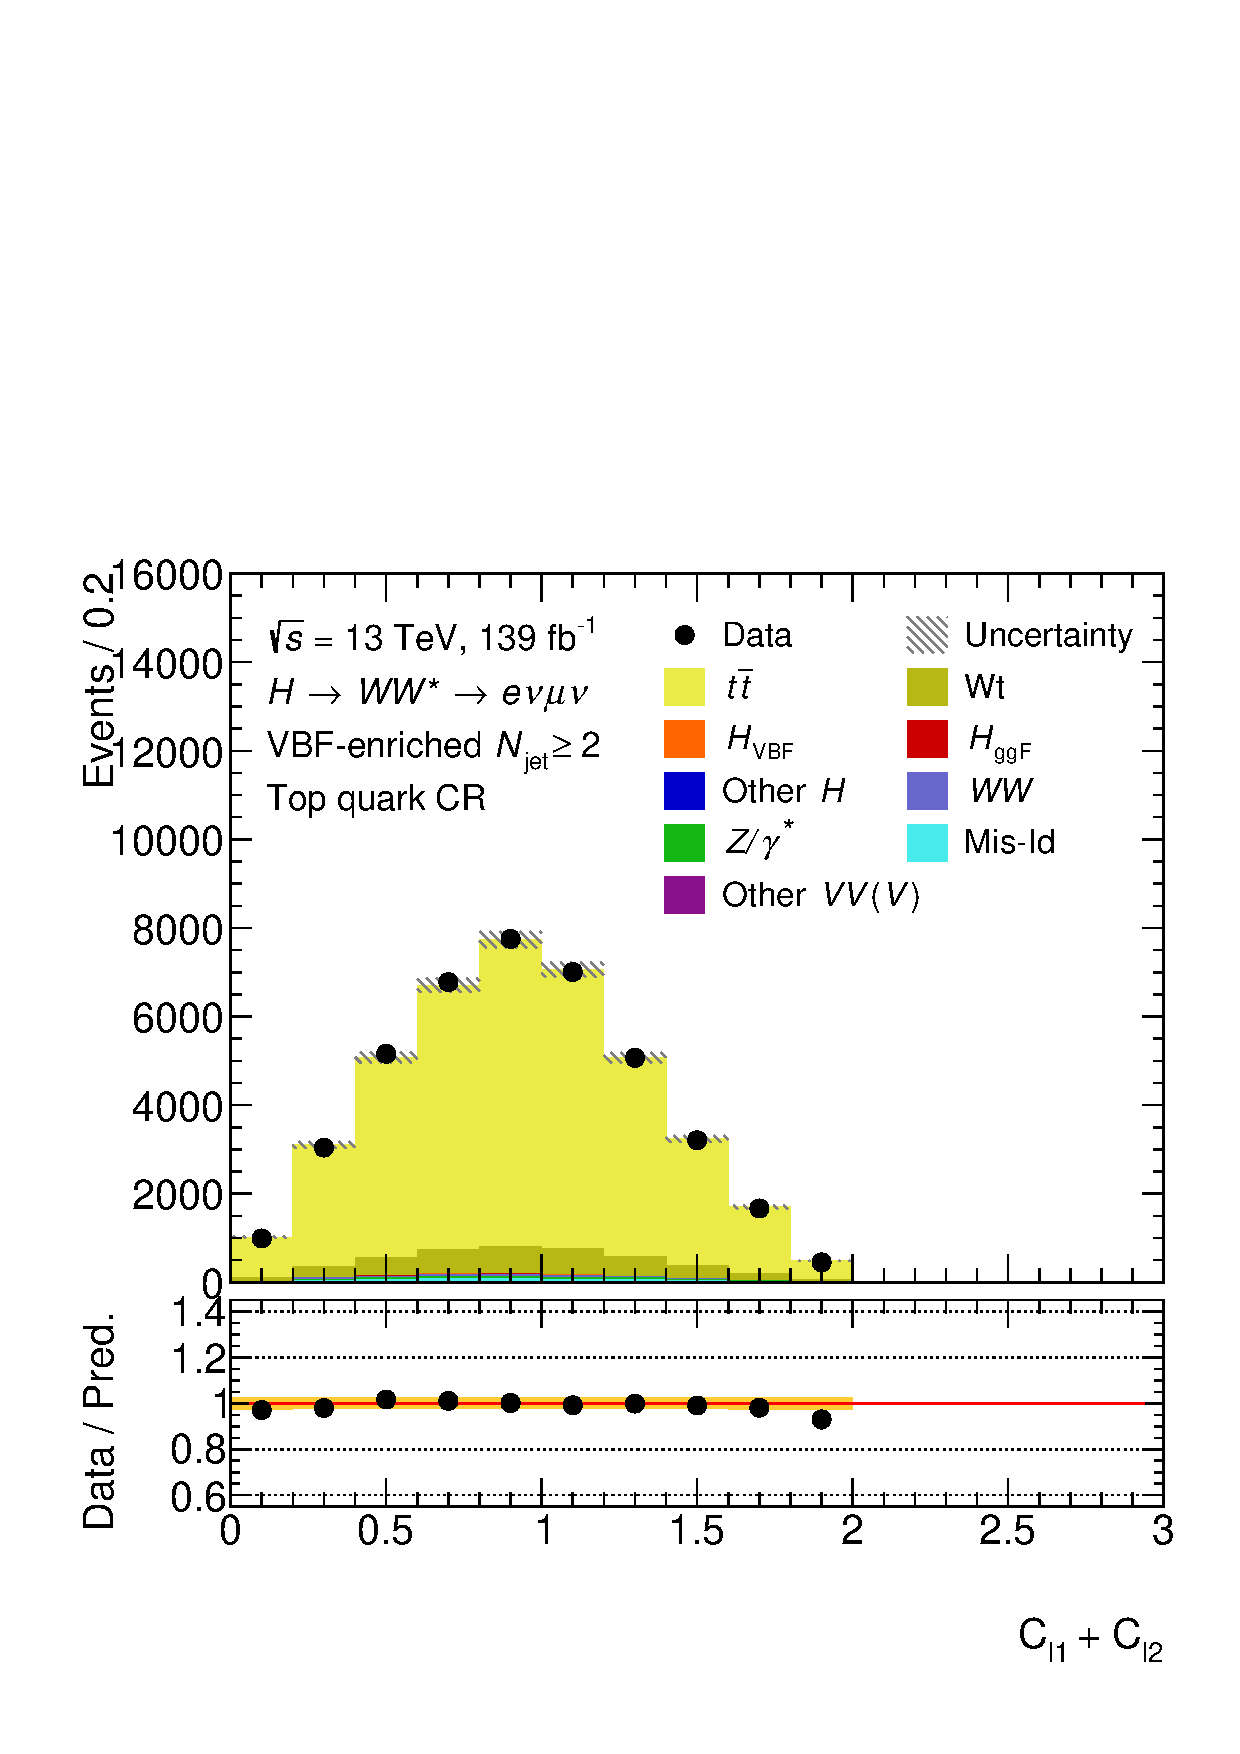
\includegraphics[width=0.490000\textwidth]{/project/ctb-stelzer/bjager/CAFoutput/results/220605-Thesis/topcr/lepcent/plots/run2-emme-CutVBF_TopControl_2jet-contOLV-lin.pdf}

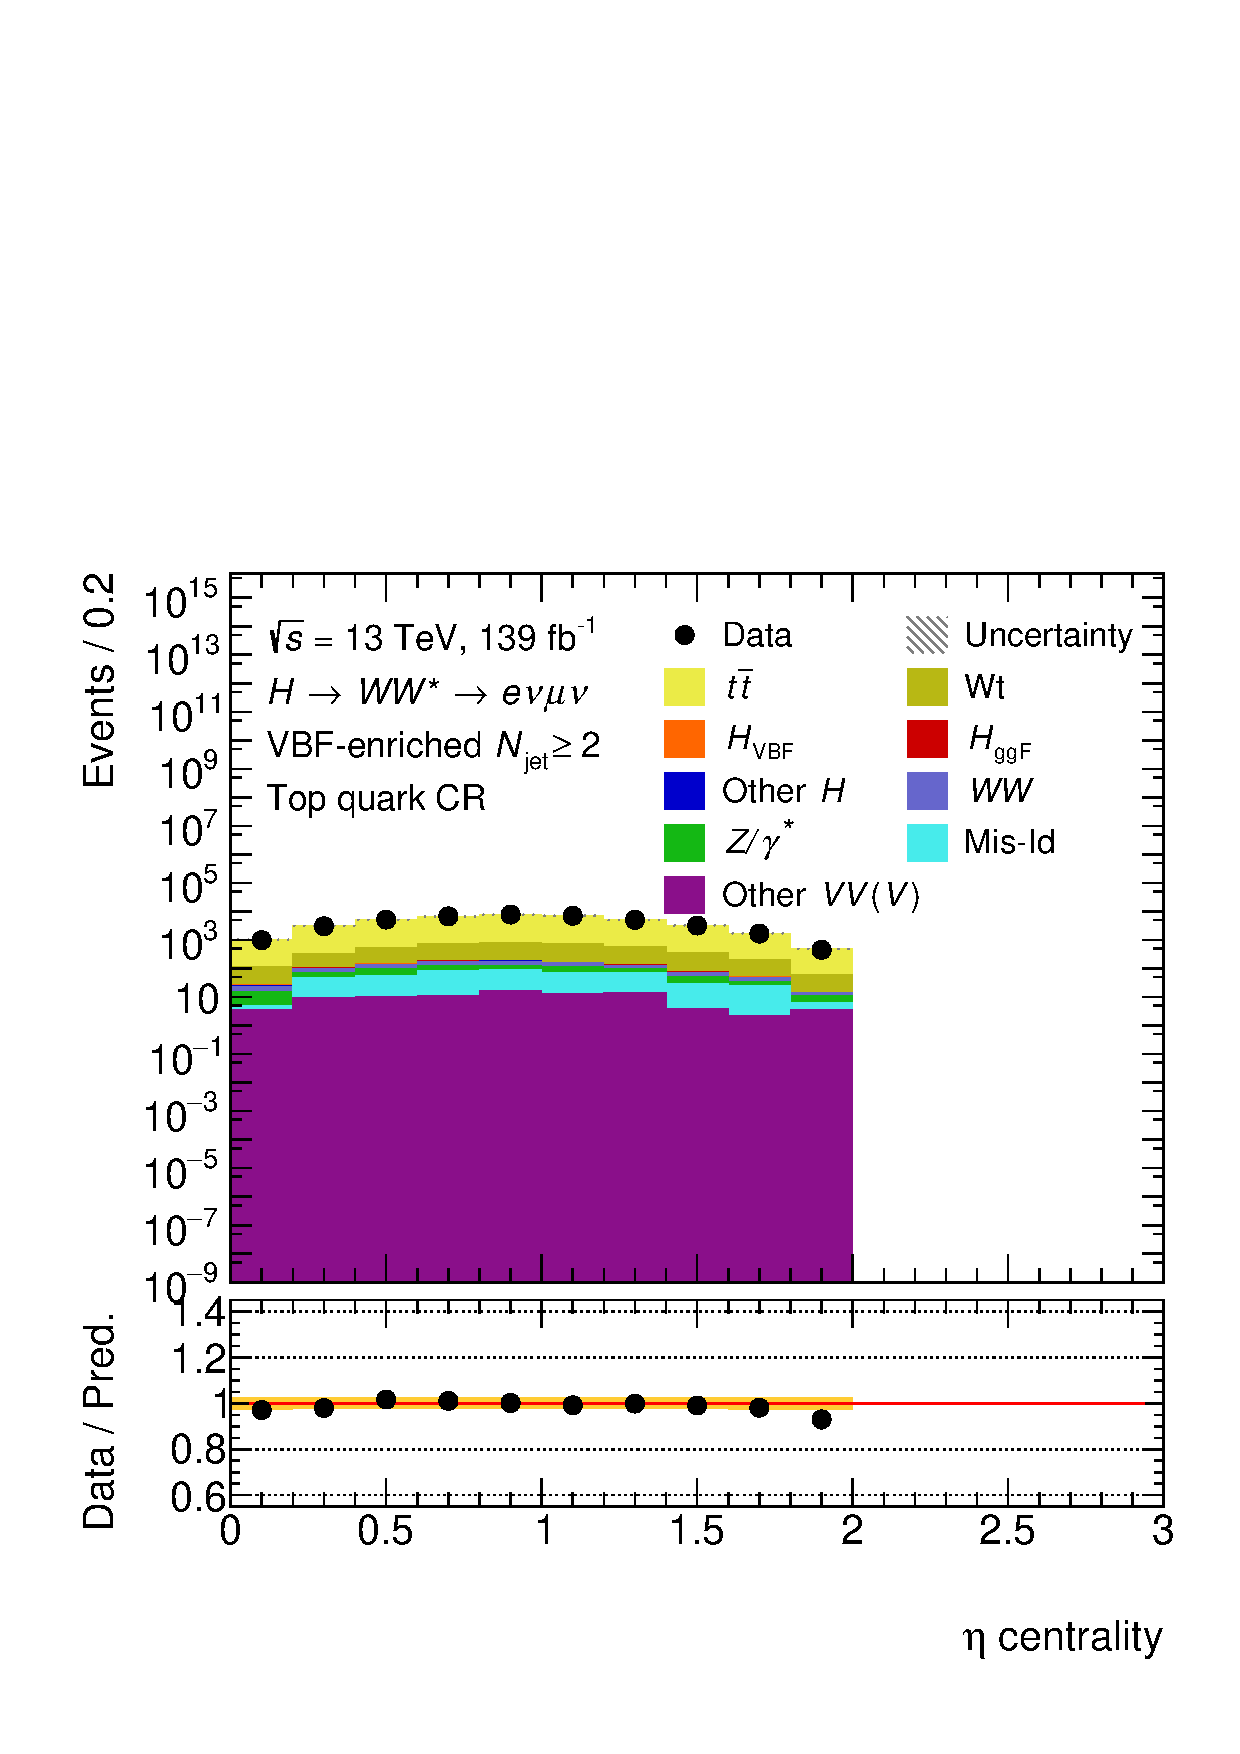
\includegraphics[width=0.490000\textwidth]{/project/ctb-stelzer/bjager/CAFoutput/results/220605-Thesis/topcr/lepcent/plots/run2-emme-CutVBF_TopControl_2jet-contOLV-log.pdf}\end{document}